\documentclass[a4paper]{article}

% Packages
\usepackage[utf8]{inputenc}
\usepackage[top=50pt,bottom=60pt,left=1in,right=1in]{geometry}
\usepackage{natbib}
\usepackage{graphicx}

%% These few lines make a distinction between latex and pdflatex calls and they
%% bring in essential packages for graphics and font handling.
%% Note that due to the \DeclareGraphicsExtensions{} call it is no longer necessary
%% to provide the the path and extension of a graphics file:
%% 
\includegraphics{diamondrule} is completely sufficient.
%%
\ifpdf%                                % if we use pdflatex
  \pdfoutput=1\relax                   % create PDFs from pdfLaTeX
  \pdfcompresslevel=9                  % PDF Compression
  \pdfoptionpdfminorversion=7          % create PDF 1.7
  \ExecuteOptions{pdftex}
  \usepackage{graphicx}                % allow us to embed graphics files
  \DeclareGraphicsExtensions{.pdf,.png,.jpg,.jpeg} % for pdflatex we expect .pdf, .png, or .jpg files
\else%                                 % else we use pure latex
  \ExecuteOptions{dvips}
  \usepackage{graphicx}                % allow us to embed graphics files
  \DeclareGraphicsExtensions{.eps}     % for pure latex we expect eps files
\fi%

\graphicspath{{figures/}{pictures/}{images/}{./}} % where to search for the images

\usepackage{microtype}                 % use micro-typography (slightly more compact, better to read)
\PassOptionsToPackage{warn}{textcomp}  % to address font issues with \textrightarrow
\usepackage{textcomp}                  % use better special symbols
\usepackage{mathptmx}                  % use matching math font
\usepackage{times}                     % we use Times as the main font
\renewcommand*\ttdefault{txtt}         % a nicer typewriter font
\usepackage{hyperref}                  % to enable \autoref
\usepackage{subcaption}                % to support captions for subfigures

% Title
\title{Volume Rendering Assignment\\2IMV20\\Technische Universiteit Eindhoven}

% Authors and group. Replace with your names and group number
\author{N. Beeren \quad H.A.C. Dias \quad G. Slavova\\Group 13}
\date{December 2020}

% Begin document
\begin{document}

\maketitle

\section{Introduction}

\subsection{Trilinear Interpolation}
\label{subsec:trilinear}

In order to achieve a smooth transition of intensity between voxels, we apply some interpolation. Given a 3D pixel coordinate $X$, we find the voxels $X_0 \ldots X_7$ such that these voxels form the vertices of a cube that contains $X$. Using the known intensities $s_{X_0}\ldots s_{X_7}$, we apply the method of trilinear interpolation to obtain an approximate intensity $s_X$ for the pixel coordinate, as desired. The implementation can be found in the method {\tt getVoxelTrilinear} of the {\tt RaycastRenderer} class. The results can be observed in \autoref{fig:trilinear}.

\subsection{Gradients}

The work related to gradients consists of two main parts:

\begin{enumerate}
  \item Computing the gradients, implemented in method {\tt compute} of class {\tt GradientVolume}.
  \item Trilinear interpolation of gradients, implemented in method {\tt getGradientTrilinear} of class\\ {\tt RaycastRenderer}.
\end{enumerate}

\noindent When the volume is first loaded, an approximate gradient is computed for all voxels, using the method described by Levoy \citep{levoy_1988}. The resulting vectors are stored in a lookup table (LUT).

To achieve a smooth transition of the gradient between voxels, we apply trilinear interpolation, similar to \autoref{subsec:trilinear}. The key difference is that we interpolate gradient vectors instead of scalar intensity values. To aid with scalar multiplication and vector addition, a few utility methods {\tt scale} and {\tt add} were implemented in the {\tt VoxelGradient} class.

\bibliographystyle{plain}
\bibliography{references}

\appendix
\section{Figures}

\begin{figure}[h]
  \centering
  \begin{subfigure}[b]{0.45\textwidth}
    \centering
    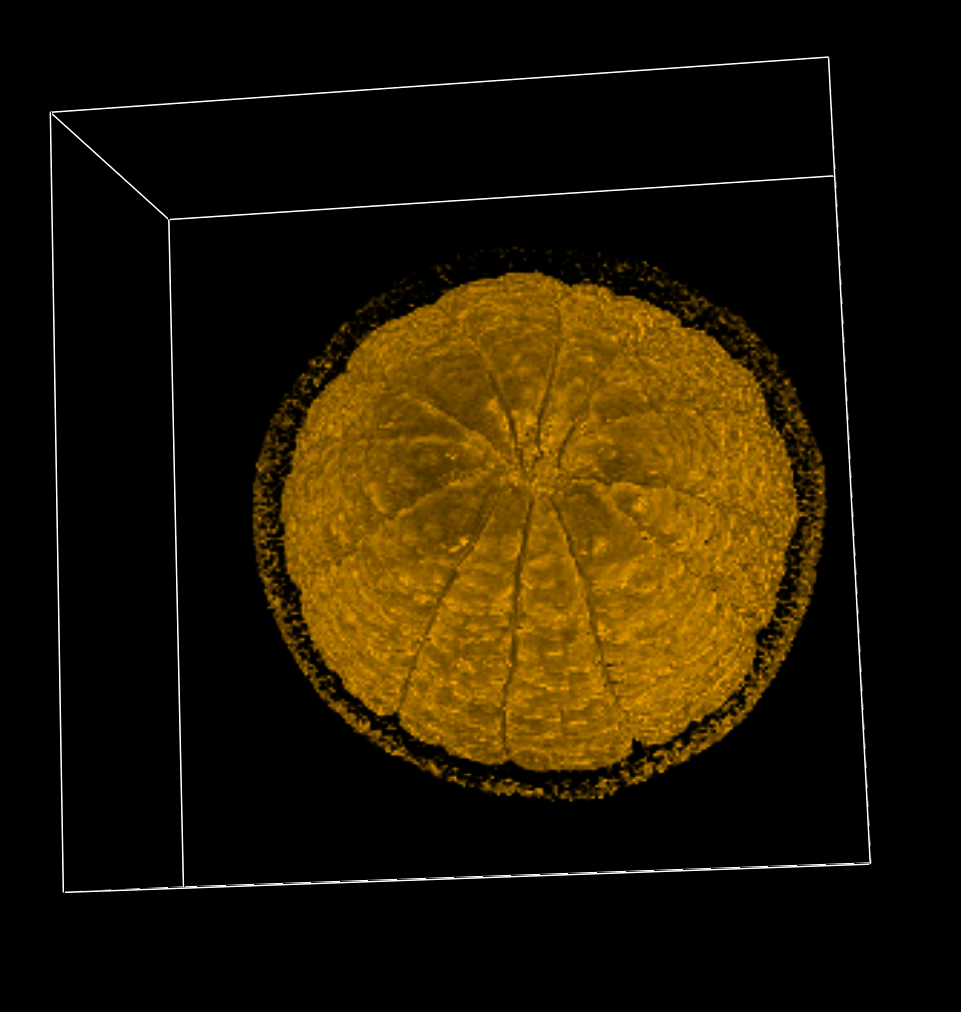
\includegraphics[width=\textwidth]{trilinear-off}
    \caption{Trilinear interpolation disabled.}
  \end{subfigure}
  \hfill
  \begin{subfigure}[b]{0.45\textwidth}
    \centering
    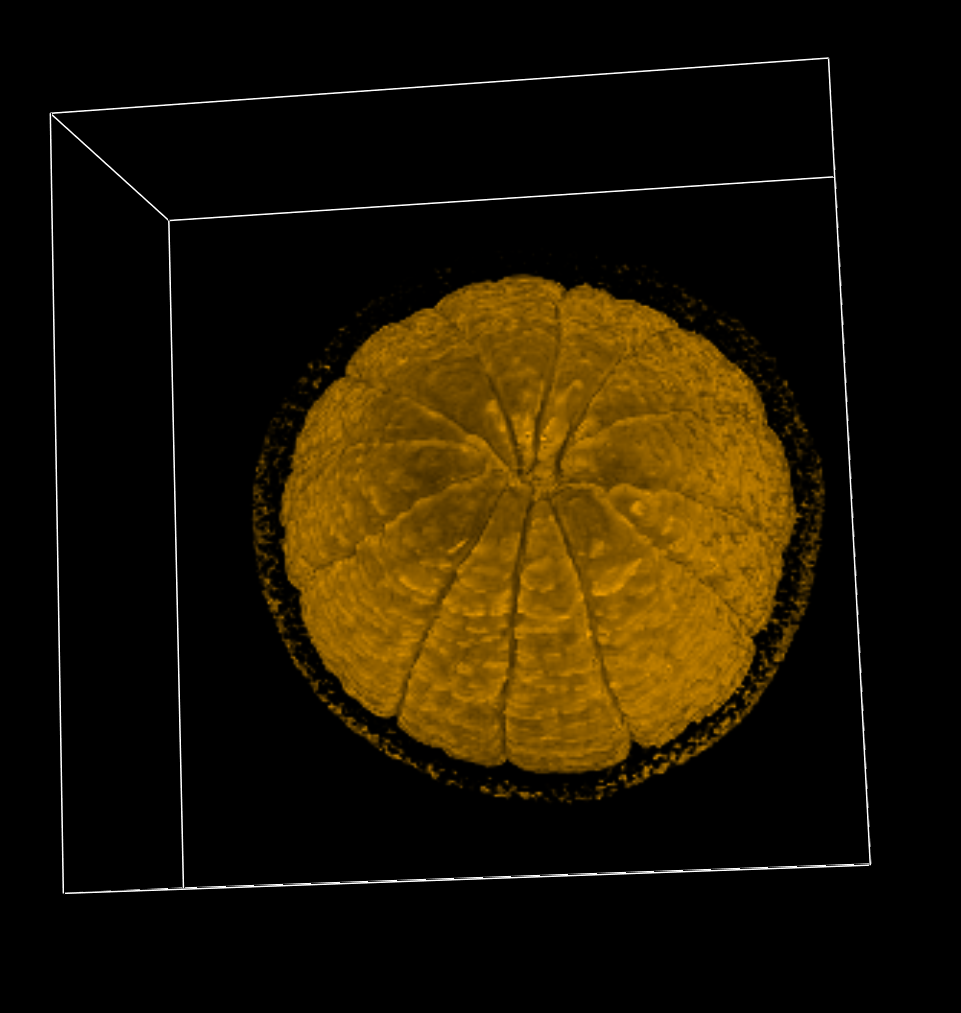
\includegraphics[width=\textwidth]{trilinear-on}
    \caption{Trilinear interpolation enabled.}
  \end{subfigure}
  \caption{Result of compositing visualization with and without trilinear interpolation on the \textit{orange} dataset.}
  \label{fig:trilinear}
\end{figure}

\end{document}
